\documentclass{beamer}
\usepackage[utf8]{inputenc}
\usepackage{tikz-cd}
\usepackage{mathtools}
\usepackage{amsmath}
\usepackage{adjustbox}

\newtheorem{remark}[theorem]{Remark}
\newtheorem{properties}[theorem]{Properties}
\newtheorem{proposition}[theorem]{Proposition}
\newtheorem{claim}[theorem]{Claim}


\usetheme{Madrid}
\usecolortheme{default}
%------------------------------------------------------------
%This block of code defines the information to appear in the
%Title page
\title[Derived Categories of Coherent Sheaves] %optional
{Derived Categories of Coherent Sheaves}

\subtitle{for Toric Varieties and GIT}

\author[Chung-Halpern] % (optional)
{Ines Chung-Halpern}

\institute[] % (optional)
{  
  LSGNT
}

\date[May 2024] % (optional)
{Mini Project 1}

%\logo{\includegraphics[height=1cm]{overleaf-logo}}

%End of title page configuration block
%------------------------------------------------------------



%------------------------------------------------------------
%The next block of commands puts the table of contents at the 
%beginning of each section and highlights the current section:

\AtBeginSection[]
{
  \begin{frame}
    \frametitle{Table of Contents}
    \tableofcontents[currentsection]
  \end{frame}
}
%------------------------------------------------------------


\begin{document}

%The next statement creates the title page.
\frame{\titlepage}


%---------------------------------------------------------
%This block of code is for the table of contents after
%the title page
\begin{frame}
\frametitle{Table of Contents}
\tableofcontents
\end{frame}
%---------------------------------------------------------

\begin{frame}{Motivation}
    \begin{itemize}
        \item (Konstevich) Homological Mirror symmetry conjecture: $D^{b}(\mathrm{Coh} (X)) \simeq \mathrm{Fuk}(X^{\vee})$ 
        %\pause
        \item (Kawamata)  DK hypothesis:  $X$ and $Y$ birational smooth projective varieties are derived-equivalent if there exists a smooth projective variety $Z$ with birational morphisms $f: Z \to X$ and $g: Z\to Y$ such that the pullbacks $f^{*}K_{X}\sim g^{*}K_{Y}$.
        %\pause
        \item We want to understand the effect of birational transformations on the structure of a derived category. 
        %\pause
        \item e.g. (Bridgeland, 2000) Birational Calabi-Yau 3-folds are derived equivalent.
    \end{itemize}
\end{frame}

\section{Dervived categories of Coherent Sheaves}

\begin{frame}{A brief introduction to $D^b (\mathrm{Coh} X)$}

Let $X$ be a scheme. Consider the abelian category $\mathrm{Coh}(X)$ of coherent sheaves on $X$, and $K(X)$ the homotopy category of complexes of objects in $\mathrm{Coh}(X)$. 

\begin{definition}
    The derived category $D^{b}(\mathrm{Coh}(X))$ on $X$ (here on out denoted $D(X)$) is a triangulated category with 
    \begin{itemize}
        \item Objects: Bounded complexes in $K(X)$
        %\pause
        \item $\mathrm{Mor}(A,B):=$ Equivalence classes of roofs $A \xleftarrow{quis} C \to B$. 
        %\pause 
        For our purposes, we will use the more usable definition $\mathrm{Hom}_{D(X)}(A,B[i]) = \mathrm{Ext}^{i}(A,B)$.
        \item an additive auto-equivalence $[1]: D(X)\to D(X)$
        \item a collection of exact triangles, of the form $$A \to B \to C \to A[1]$$
    \end{itemize}

\end{definition}    
\end{frame}



\begin{frame}{Fourier Mukai Transforms}
\begin{definition}
Given $\mathcal{E}\in D^b(X\times Y)$, we define the Fourier Mukai Transform
\begin{align*}
\Phi_\mathcal{E} : D^{b}(X) &\to D^b(Y) \\
\mathcal{F} &\mapsto p_{*}(\mathcal{E}\otimes^L q^*\mathcal{F})
\end{align*}
where $q:X\times Y\to X$, $p:X\times Y\to Y$ are the projections.    
\end{definition}

\end{frame}


\begin{frame}{Semi-orthogonal Decompositions}
    \begin{definition}
        A full subcategory is admissible if its inclusion $i_*$ admits both a left and right adjoint $i^*$ and $i^!$ respectively
    \end{definition}
    %\pause
    \begin{definition}
        For a sequence of admissible subcategories $A_{1}, \dots, A_{k}\subset D(X)$, we say $D(X)$ has a semi-orthogonal decomposition $$D(X) = \left< A_1,\dots,A_k \right> $$ if $D(X)$ is generated by elements of $A_1,\dots,A_k$, and there are no morphisms from right to left, i.e. for $j<i$, $$A_{j}\subset A_i^\perp$$
    \end{definition}
\end{frame}

\begin{frame}{Semi-orthogonal Decompositions}
    \begin{example}{Beilinson's exceptional collection}
        $$D(\mathbb{P}^{n})= \left< \mathcal{O}, \mathcal{O}(1),\dots,\mathcal{O}(n) \right> $$ where each $\left< \mathcal{O}(i) \right>\simeq D(\left\{ pt \right\})$. This is an example of a full exceptional collection, which is a stronger special case of a SOD. 
    \end{example}
\end{frame}

\begin{frame}{Blow-up Formula}
Let  $Z$ be a smooth subvariety of $Y$ of codimension $c$. Consider the blow-up $X = \mathrm{Bl}_{Z}(Y)$,  with $E = \mathbb{P} (\mathcal{N}_{Z/Y})$

\begin{figure}[!h]
    \centering
    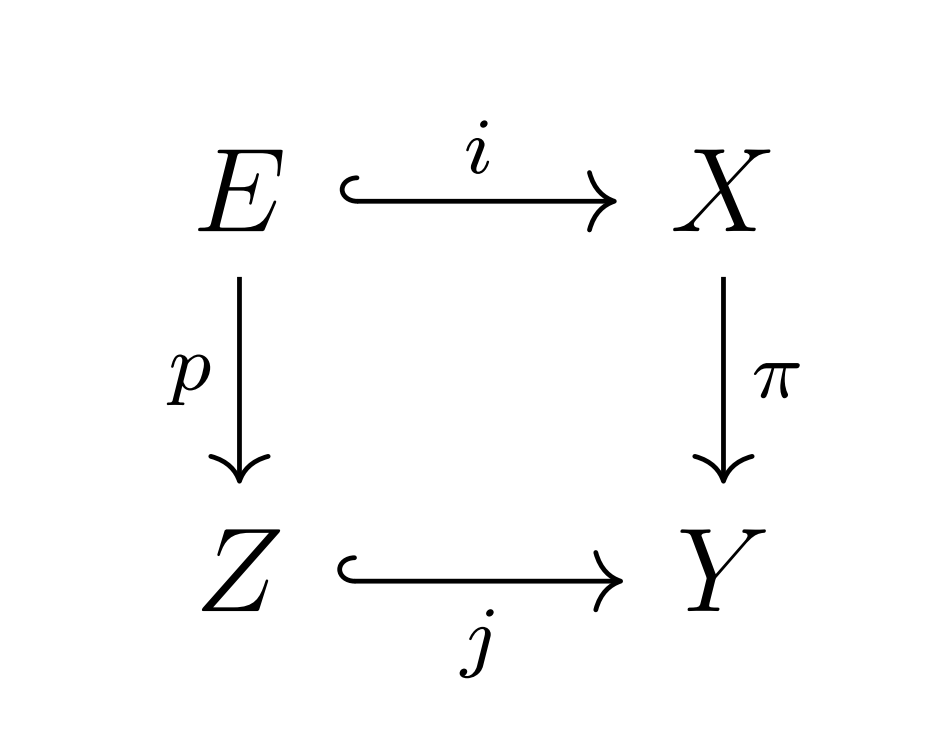
\includegraphics[width = 3cm]{blow up.png}
\end{figure}
%\pause
For $k\in \mathbb{Z}$ we can consider $\mathcal{O}_{E}(kE)$ as an element of $D(Z\times X)$
\vspace{0.3cm}
%\pause

We get a collection of FM transforms $\Phi_k$ with kernel $ \mathcal{O}_{E}(kE)$.
\vspace{0.3cm}
%\pause

$\Phi_{k}$ is fully faithful, and $\Phi_{k} (D(Z))$ is an admissible subcategory of $D(X)$. 

\end{frame}

\begin{frame}{Blow-up formula}
    Define  $\mathcal{D}_{-k}=\mathrm{Im}(\Phi_{k})$ and $\mathcal{D}_{0}= \pi^{*}D(Y)$ 
%\pause
\begin{theorem}
    Let $Z$ be a smooth subvariety of $Y$ of codimension $c$, and $X = \mathrm{Bl}_{Z}(Y)$. Then we have a semi orthogonal decomposition $$D(X) = \left< \mathcal{D}_{-c+1},\dots,\mathcal{D}_{-1}, \mathcal{D}_0 \right> $$
\end{theorem}
\end{frame}

\section{Toric GIT}


\begin{frame}{Toric GIT}
Let $M = \mathrm{Hom}(T^{n}, \mathbb{C}^*)$, and $N = M^{\vee}$. Recall that toric varieties are determined by their fan in $N_\mathbb{R}$, with an exact sequence and its dual
\begin{align}
0 \to \mathbb{L}\to &\mathbb{Z}^{m}\xrightarrow{\rho}N \to 0 \\
0 \to M \to (&\mathbb{Z}^{m})^{\vee} \xrightarrow{Q} \mathbb{L}^{\vee}\to {0}
\end{align}
%\pause

\begin{itemize}
    \item The map $Q$ describes an action of $(\mathbb{C}^{*})^n$ on the vector space $\mathbb{C}^m$, given by a $n\times m$ weight matrix, so we can form a GIT quotient.
    %\pause
    \item The semi-stable locus is given by a choice of character $\chi$ in $\mathbb{L}^\vee$ 
    \begin{align*}
        X^{ss}_\chi &= V(Irr_\chi )\\
        Irr_{\chi}&= (x_{i_{1}},\dots,x_{i_{r}} \mid \chi \in \left< q_{i_{1}},\dots,q_{i_{r}}\right>_{+} )
    \end{align*}
    %\pause
    \item The toric variety $X_\chi$ is the quotient $$X_\chi = \mathbb{C}^{m}//_{\chi}T^{n}:= \left(\mathbb{C}^{m}-X^{ss}_\chi)\right)  /T^n$$
        
\end{itemize}
\end{frame}

\begin{frame}{Example}

%Different stability conditions define different toric varieties


Let $(\mathbb{C}^{*})^{2}= T^2$ act on $V = \mathbb{C}^4$ by 
\begin{align*}
(\lambda,\mu)(x_1,x_2,x_3,x_{4}) &= \left( \lambda x_{1}, \lambda x_{2},\mu x_{3}, \frac{\mu}{\lambda^{2}}x_4 \right)\\
Q = \begin{pmatrix}1&1&0&-2 \\ 0&0&1&1\end{pmatrix} & \qquad \det V = \sum q_i = (0,2)^T
\end{align*}
%\pause

The weight matrix forms a fan in $\mathbb{L}^\vee$, called the \emph{secondary fan}, which forms a wall-and-chamber decomposition.  Any character in the same chamber gives the same semi-stable locus. 

\begin{figure}[!h]
    \centering
    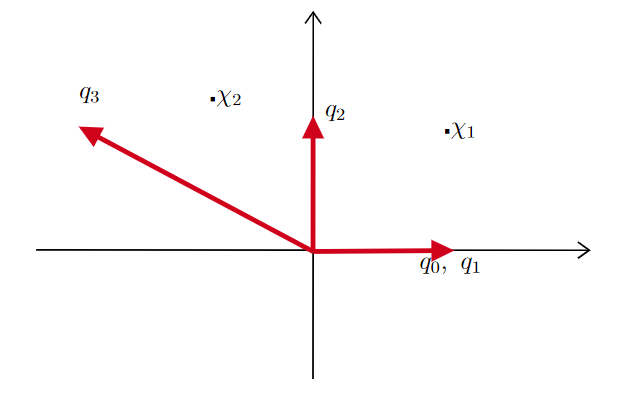
\includegraphics[width = 5cm]{secondary fan.png}
\end{figure}
\end{frame}

\begin{frame}{Example (Cont.)}
    
\begin{figure}[!h]
    \centering
    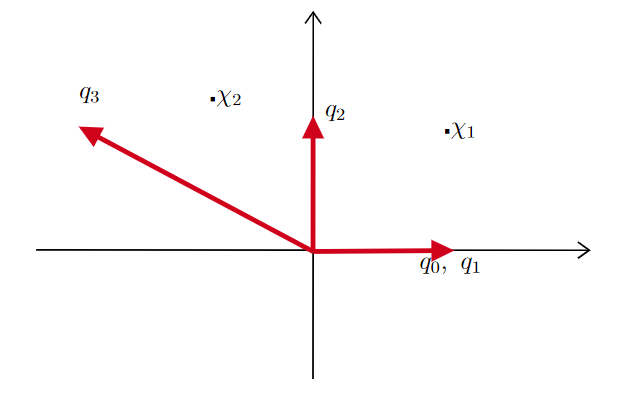
\includegraphics[width = 3.75cm]{secondary fan.png}
\end{figure}

    %\pause
\begin{enumerate}
    \item $X_{1}= \mathbb{C}^{4}//_{\chi_{1}}T^{2}= \mathbb{P}(\mathcal{O}_{\mathbb{P}^{1}}\oplus \mathcal{O}_{\mathbb{P}^{1}}(2)) = \mathbb{F}_2$
    %\pause
    \item $X_{2}= \mathbb{C}^{4}//_{\chi_{2}}T^{2}= \mathbb{P}(1,1,2)$
\end{enumerate}
%\pause
The wall-crossing from $X_2$ across $\langle q_2 \rangle_+$ is the blow up of $\mathbb{P}(1,1,2)$ at its unique singular point. 
%\pause

\begin{remark}
    Toric wall-crossings give other birational transformations. In fact, the Toric MMP is realised as a sequence of wall-crossings in the secondary fan, crossing 'away' from $\det V$. 
\end{remark}
  
\end{frame}


\begin{frame}{Wall crossing formula}
    
    As it turns out, these wall crossings manifest very nicely in the derived categories, by inducing a semi orthogonal decomposition.
    \vspace{0.3cm}
    %\pause

    A wall $W$ in $\mathbb{L}^\vee$ has a normal 1-PS $\lambda_W$ in $\mathbb{L}$. 

    \vspace{0.3cm}

    Define $\kappa := (\det V)(\lambda_W) $ ($\geq 0$ by choice of orientation of $\lambda_W$), so $\lambda_W$ points to the chamber with the 'bigger' quotient.
%\pause

    \vspace{0.3cm}
    We can define  a strictly lower dimensional subvariety $Z$ constructed from a 'sub' toric GIT problem: %\pause

\begin{itemize}
    \item  Take the vector space $\left< W \right>$ as the new character lattice
    %\pause

    \item The new weight matrix being the columns of $Q$ orthogonal to $\lambda_W$, defining an action on $V^{\lambda_{W}}$ be the invariant locus of $\lambda_W$
    %\pause

    \item $Z$ is the GIT quotient of $V^{\lambda_{W}}$ defined by a character $\chi_W$ on the ray generated by $W$. 
\end{itemize}

\end{frame}



\begin{frame}{Wall crossing formula}

\begin{theorem}[Halpern-Leistner--Shipman,  Ballard-Favero-Katzarkov]
    Given a wall separating two adjacent chambers $C_+$ and $C_-$ in the secondary fan, assume we have labelled the chambers such that $C_+$ lies on the side of the wall $\lambda_W$ is pointing. 
If $\kappa >0$, we have an SOD $$
D(X_{+})= \left< D(X_{-}), D(Z),\dots,D(Z) \right> 
$$with $\kappa$ copies of $D(Z)$.
If $\kappa=0$ the wall crossing induces a flop, and we have an equivalence $$
D(X_{+})\simeq D(X_{-})
$$
\end{theorem}
    
\end{frame}


\begin{frame}{Wall-crossing Formula}
    \begin{example}[ Beilinson's exceptional collection]
Consider the usual action of $\mathbb{C}^*$ on $V = \mathbb{C}^{n+1}$. So the weights are $\begin{pmatrix}1 & 1 &\dots &1\end{pmatrix}$, with $\det V = n+1$. Wall crossing to $X_{-}=\emptyset$, we get $$D(\mathbb{P}^{n})= \left< pt, \dots,pt \right> = \left< \mathcal{O}, \dots,\mathcal{O}(n) \right>$$ with $n+1$ copies of $D(pt)$, which retrieves Beilinson's exceptional collection.
\end{example}
%\pause
\begin{example}[Blow-up of $\mathbb{C}^2$]
Consider the action of $\mathbb{C}^{*}$ on $\mathbb{C}^3$ with weights $(1,1,-1)$. 
%\pause
There are two quotients: $X_+ =  \mathcal{O}(-1)_{\mathbb{P}^{1}}$  or $X_{-}= \mathbb{C}^2$
The wall-crossing formula gives  $$D(\mathcal{O}(-1)_{\mathbb{P}^{1}})= \left< \mathbb{C}^{2}, pt \right> $$ which recovers Orlov's blow-up formula.

\end{example}
\end{frame}


\section{Window Shifts and Spherical Twists}

\begin{frame}{Flops}

Now suppose $\mathbb{C}^*$ now acts on $V = \mathbb{C}^4$  with coordinates $x_{1}, x_{2}, y_{1},y_{2}$, and weight matrix $$Q = \begin{pmatrix}1&1&-1&-1\end{pmatrix}$$ 
%\pause

This defines two chambers in the secondary fan: $\chi_{+}>0$ and $\chi_{-}<0$, so we get unstable locus $x_{1}= x_{2}= 0$ and $y_{1}= y_{2}=0$. Hence $$
X_{+}\simeq \mathcal{O}(-1)_{\mathbb{P}^{1}}^{\oplus_{2}}\simeq X_-
$$related by a flop along the zero section $\mathbb{P}^1_{x_1 , x_2}$.
%\pause
\vspace{0.3cm}

Clearly these are derived equivalent, but the flop gives us a family of autoequivalences indexed by $\mathbb Z $, called \emph{spherical twists}. 
\end{frame}

\begin{frame}{Window shifts}

$X_+$ and $X_-$ are both substacks of the quotient stack $\mathfrak{X} = [\mathbb{C}^4 / \mathbb{C}^*]$, with inclusions $i_{\pm} : X_\pm -> \mathfrak{X}$. 

%\pause
\vspace{0.3cm}

The subcategory $\mathcal{W}_t = \left<\mathcal{O}(t),\mathcal{O}(t+1) \right> \subseteq D(\mathfrak{X})$ is called a \emph{window subcategory}.

In fact, the restriction $i^*_\pm \big|_{\mathcal{W}_t}: \mathcal{W}_t \to D(X_\pm )$ is an equivalence. Define 
$$\psi_{t}:= i_{+}\circ i_{-}^{*}: \mathcal{D}(X_{-})\to \mathcal{W}_t \to \mathcal{D}(X_{+})$$
Then the we get the autoequivalence 
$$\Phi_{t}:= \psi_{t+1}^{-1}\psi_{t}: \mathcal{D}(X_{-})\to \mathcal{W}_t \to D(X_+ ) \to \mathcal{W}_{t+1} \to \mathcal{D}(X_{-})$$
By passing through one window, then back through another. This is called the \emph{window shift autoequivalence}.
\end{frame}

\begin{frame}{Spherical Twists}
    \begin{definition}
        An object $\mathcal{E} \in D(X)$ is \emph{spherical} if: 
        \begin{itemize}
            \item $\mathcal{E} \simeq \mathcal{E} \otimes \omega_X $, and
            \item $\mathrm{Ext}^i (\mathcal{E}, \mathcal{E}) = \begin{cases}
                \mathbb{C}& \quad i=0, \mathrm{dim}(X) \\
                0&\quad \text{otherwise}
            \end{cases}$
        \end{itemize} 
    \end{definition}

%\pause

    \begin{definition}
        The \emph{spherical twist} around $\mathcal{E}$ is the FM transform on $D(X)$  with kernel $C\left(\mathcal{E}^\vee \boxtimes \mathcal{E} \to \mathcal{O}_\Delta \right)$, which sends $\mathcal{F}\in D(X)$ to the cone 
        
        $$C\left(\mathrm{RHom}(\mathcal{E},\mathcal{F}) \otimes \mathcal{E}\to \mathcal{F} \right ).$$

        The \emph{inverse spherical twist} sends $\mathcal{F}\in D(X)$ to the cone 
        $$C \left(\mathcal{F}\to \mathrm{RHom}(\mathcal{E},\mathcal{F})^\vee \otimes \mathcal{E}  \right)$$
    \end{definition}
\end{frame}


\begin{frame}{Window Shifts are Spherical Twists}
    \begin{theorem}[Segal]
        The window shift functor $\Phi_{t}$ is an inverse spherical twist around the spherical object $\mathcal{O}_{\mathbb{P}^1_{x_1 , x_2}}(t)$.
    \end{theorem}
%\pause

    \begin{remark}
        This is just one example of a much more general phenomenon of flop autoequivalences appearing as spherical twists. Donovan-Segal generalised this result to Grassmanian Flops, and Halpern-Leistner--Shipman showed that window shift functors being the same as spherical twists holds for all flops induced by a certain kind of wall-crossing.
    \end{remark}
\end{frame}
\begin{frame}{}
    Thanks for listening!
\end{frame}
\end{document}
